\section{Robotics Environment Descriptions}

We have two testbed environments: one with the simplified task description and the full task description. We primarily use the simplified environment to test and prune the algorithms quickly. If the model solves the simplified environment, we move forward to try it in the full environment. Those two descriptions deviate in terms of action, observation, reward, and curriculum definition \ref{tab:envpars}, \ref{tab:currpars}. 

The simplified environment has fewer action dimensions to control compare to the full environment. A total of three-dimensional action controls the x, y coordinates translation, and yaw rotation. Hence, every timestep it receives a fixed size of downward z-axis movement. Similar to Quillen et al. and Breyer et al., our gripper also automatically closes when it reaches a certain height threshold.

The full environment, on the other hand, has full control over all dimensions. The gripper receives five-dimensional action to control cartesian coordinates (x, y, z), yaw rotation, and the gripper open/close in the full environment. 

Observation from the environment differs as well, based on the task description. In the simplified scenario agent only receives the hundred-dimensional encoded depth image. Whereas, in the full scenario, the agent gets the actuator width and the hundred-dimensional encoder output. [\todo{yaz bir seyler daha} ]

We used a custom shaped reward function for the environment setting. In the simplified environment, a sparse reward definition was used. \todo{Better}

Curriculum strategy guides the agent to a more challenging environment based on the agent's success rate. In our case, curriculum switch happens both on simplified and full environment definition at a \(70\%\) success rate. This switch triggers an increase of difficulty on the environment's curriculum parameters such as max object count, object spawned area, and terminating object height. More detailed information given in the below table in \ref{tab:currpars}

\todo{Explain Curr Tables}

\begin{figure}[htbp]
    \centering
    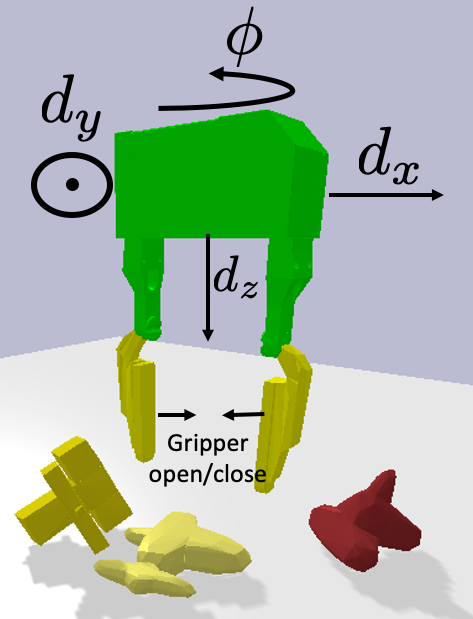
\includegraphics[width=0.3\linewidth]{figures/freedomDim.png}
\caption{Full environment freedom of movement} \label{fig:breyer}

\end{figure}


\begin{table}[htbp]
    \resizebox{\textwidth}{!}{
    \begin{tabular}{lllll}
    \toprule
     Env. Description     & Action Space & Observation                                           & Reward        & Discount Factor \\ \midrule % \hline
               Full       & 5            &  \shortstack{Encoder  + \\ Actuator Width or \\ RGBD \\ Depth} & Shaped Reward & 0.99  \\  \midrule % \hline
               Simplified & 3            & Encoder                                        & Binary Reward & 1.0    \\      %\hline
    \bottomrule
\end{tabular}}
\caption{Different paramters of Simplified and Full environment definitions \label{tab:envpars}}
\end{table}

\begin{table}[htbp]
    \resizebox{\textwidth}{!}{
    \begin{tabular}{llllll}
    \toprule
    Env. Description  & Curr Steps & Curr Success Thresh. & Robot Height & Max Objects & Object Area \\ \midrule
    Full                    & 8                & 0.7                          & [0.15, 0.25] & [3, 5]       & [0.01, 0.1]  \\ \midrule
    Simplified              & 4                & 0.7                          & [0.17, 0.27] & [3, 5]       & [0.01, 0.1]  \\ 
    \bottomrule
    \end{tabular}}
    \caption{Curriculum Parameters of Simplified and Full environment descriptions \label{tab:currpars}}
\end{table}